\chapter{Secure Device Identity}

% maybe expand and clarify some points


A secure device identifier (DevID) is defined as an identifier that is cryptographically bound to a device \cite{DevIDSpec-IEEE}. A DevID must not be transferable from one device to another and must be stored in a way that protects it from modification. Since the TPM is a secure Root of Trust for Storage and protects keys against compromise, TPM keys are an ideal choice for DevIDs. A device with TPM-based DevID capabilitities includes at least one Initial Device Identifier (IDevID).  An IDevID is intended to be long-lived and usable for the lifetime of the device. IDevIDs are installed by OEMs in TPM-containing devices at manufacturing time. Additionally, a device with DevID capabilitities may support the creation of Locally Significant Device Identifiers (LDevIDs) by the end user (i.e., the Owner). LDevIDs are not expected to be long-lived because an Owner may create new LDevIDs as often as they need.
%An LDevID must not be transferable to a device with a different IDevID without knowledge of the private key used to produce the cryptographic binding. 

When using a TPM key for secure device identity, there are restrictions on the attributes that it can have in order to enforce the best security practices. The \verb|Sign| attribute must be set and the \verb|Decrypt| attribute not set. Furthermore, the \verb|FixedTPM| attribute must be set because it is of paramount importance that a DevID never be duplicated, transferred, or copied. On the other hand, the \verb|Restricted| attribute is optional. When the \verb|Restricted| attribute is set, such a key is called an attestation key (AK). This DevID gets its special name due to its unique ability to be used as a parent node in a chain of certificates. This idea is discussed in detail in the following section. The acronym AK is prefixed by the letter I or L denoting Initial or Locally Significant respectively. 
\begin{table}[h]
  \begin{center}
    \scriptsize 
    \sffamily
    \renewcommand{\arraystretch}{1.5}
    \begin{tabular}{ |c|c|c|c|c|c|c| }
      \hline
      Key & Type & \verb|FixedTPM| & \verb|Signing| & \verb|Decrypting| & \verb|Restricted| & Creator \\
      \hline
      \hline
      EK & Primary       & X &   & X & X & TPM Manufacturer \\
      \hline
      IAK & Primary      & X & X &   & X & OEM \\
      \hline
      IDevID & Primary   & X & X &   &   & OEM \\
      \hline
      LAK & Ordinary     & X & X &   & X & Owner \\
      \hline
      LDevID & Ordinary  & X & X &   &   & Owner \\
      \hline
    \end{tabular}
    \caption{Key Requirements and Recommendations}
    \label{fig:req_and_recs}
  \end{center}
\end{table}
 OEM-installed DevIDs (i.e., IAKs and IDevIDs) should be Primary keys so that they may be recoverable by the Owner. Since an Owner cannot provision new IAKs or IDevIDs on their device, these keys should be able to be recreated during the lifetime of the TPM or more precisely during the lifetime of the TPM’s Primary Seed to avoid the problematic loss of these essential identifiers. An IAK should be used only for the certification of new DevIDs and even then should only be used sparingly to limit the chances of compromise. Similarly, an IDevID should be used sparingly but instead for device authentication in an enterprise network. Since an Owner may create LAKs and LDevIDs as often as need, these DevIDs may be used freely. Although, it is still recommended that any given DevID---LAK and LDevID included---be used in only a single application. An LAK is intended to be used for the purposes of attestation as well as for the certification of new DevIDs. While an LDevID is intended to be used for any general device authentication purposes.

The issuers of device identity certificates are known as Certificate Authorities (CAs). CAs are further identified by the creator of the keys that they certify (i.e., the CA that issues certificates for IAKs and IDevIDs is known as the OEM's CA and the CA that issues certificates for LAKs and LDevIDs is known as the Owner's CA). All CAs should support a standard certificate transport protocol that provides confidentiality, integrity, and protection from replay attacks \cite{DevIDSpec-TCG}. These transport protocols are outside the scope of this paper. This work assumes CAs to be following this recommendation precisely. The OEM's CA must carefully verify the attributes and TPM residency of a key before signing a certificate due to the important security and identity implications provided by these certificates. The Owner's CA ideally should also verify the attributes and TPM residency of a key before signing a certificate. The attribute requirements displayed in Table \ref{fig:req_and_recs} is modeled as a collection of functions. Each function takes a public key as input and returns a proposition. If a CA issues a certificate, then applying the corresponding function on the subject DevID should result in the value \verb|True|. These functions are useful in the verifications performed in Chapter 4.
\begin{figure}[h]
\begin{lstlisting}[language=Coq]
Definition endorsementKey (k : pubKey) : Prop :=
  match k with
  | Public _ Restricting NonSigning Decrypting Fixing => True
  | _ => False
  end.

Definition attestationKey (k : pubKey) : Prop :=
  match k with
  | Public _ Restricting Signing NonDecrypting Fixing => True
  | _ => False
  end.

Definition devidKey (k : pubKey) : Prop :=
  match k with
  | Public _ NonRestricting Signing NonDecrypting Fixing => True
  | _ => False
  end.
\end{lstlisting}
\caption{Model of Key Attribute Requirements}
\end{figure}
 




\section{Certificate Chain}

A chain of certificates can be used to verify a chain of trust to some trust anchor \cite{DevIDSpec-TCG}. Since IAK certificates provide definitive evidence to a remote entity that a key belongs to a specific device, an IAK certificate typically acts as this trust anchor. 
Although certification of an IAK relies on the EK certificate, an IAK certificate is still sufficient to act alone as this trust anchor. Note that the TPM Manufacturer's method for creation of an EK certificate is outside the scope of this paper since an EK is not a DevID (an EK certificate identifies a TPM not a device). 
%Although this evidence's legitimacy is technically reliant on that of the EK certificate, this work trusts all valid EK certificates at face value.


Since a key with the \verb|Restricted| attribute set has the ability to prove that some unknown key is resident in the same TPM as itself, AKs are used in the certification of new DevIDs. This means that AK certificates may be parent nodes in a chain of certificates. 
In issuing an IAK certificate, the OEM's CA makes an assertion that is a primary security dependency for all future enrollment of DevIDs. 
To demonstrate that some non-IAK DevID belongs to  a specific device, one must provide a chain of certificates which links that DevID's certificate to an OEM-provided root certificate.
The underlying security implications provided by a chain of certificates is formed by the protocols which provision these certificates. Specifically, the Proof of Residency and Chain of Trust lines in Figure \ref{fig:cert_rel} are a direct consequence of the assurances provided by the respective provisioning protocols.



%enrollment of all DevIDs is reliant, either directly or indirectly, on an IAK certificate. Figure \ref{fig:cert_rel} shows that the IDevID, LAK, and LDevID may all be linked back to the IAK. We trust that an EK certificate provides definitive evidence that the EK resides within the specific TPM.

 
\begin{figure}[h]
  \begin{centering}
  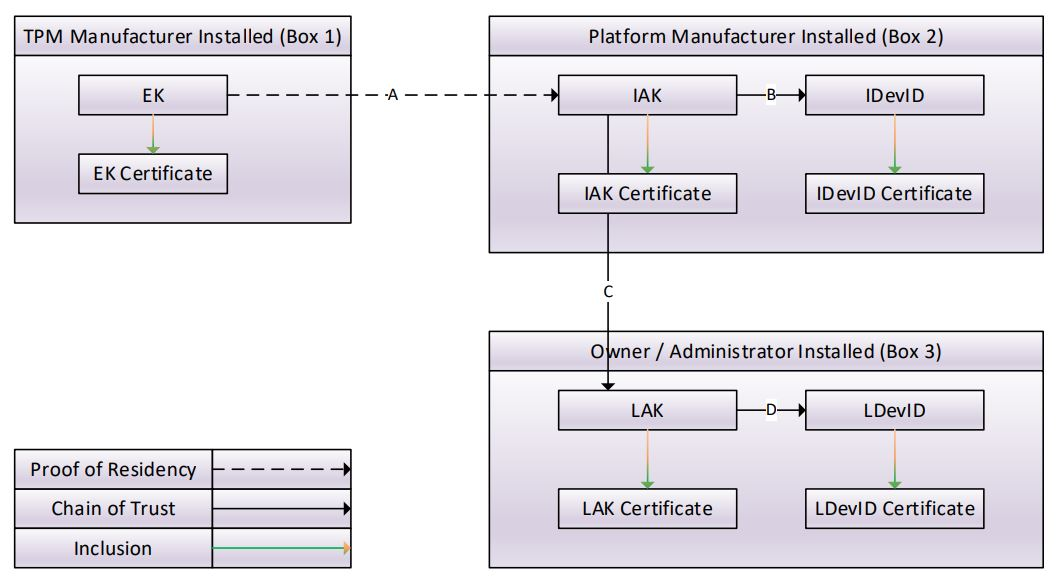
\includegraphics[width=\linewidth]{chap_3_figures/certificateRelationships.jpg}
  \par\end{centering}
  \caption{Key and Certificate Relationships \cite{DevIDSpec-TCG}}
  \label{fig:cert_rel}
\end{figure}
\begin{itemize}[itemsep=0pt,parsep=0pt,partopsep=0pt]
  \item \textsf{Box 1}: The EK certificate is signed by the TPM Manufacturer's CA and binds the EK to a specific TPM.
  \item \textsf{Line A}: The IAK is verified by the OEM's CA to have the correct key properties and to be resident in the same TPM as the EK.
  \item \textsf{Line B}: The IDevID is verified by the OEM's CA to have the correct key properties and to be resident in the same TPM as the IAK.
  \item \textsf{Box 2}: The IAK certificate and IDevID certificate is signed by the OEM's CA and binds the IAK and IDevID to a specific device.
  \item \textsf{Line C}: The LAK is verified by the Owner's CA to have the correct key properties and to be resident in the same TPM as the IAK.
  \item \textsf{Line D}: The LDevID is verified by the Owner's CA to have the correct key properties and to be resident in the same TPM as the LAK.
  \item \textsf{Box 3}: The LAK certificate and LDevID certificate is signed by the Owner's CA.
\end{itemize}

\vspace{2em}
Although, Figure \ref{fig:cert_rel} shows the relationships between keys and certificates for exactly one of each type of DevID, in practice, there often exists multiple of each type of DevID. Due to algorithm agility, an OEM usually installs multiple IAKs and IDevIDs with varying algorithms and sizes. While an IDevID is always linked directly to an IAK, an LAK or LDevID may be linked directly to either an IAK or LAK. Specifically this means that an LAK certificate may be used in the certification procedure for LDevIDs and additional LAKs creating an arbitrarily long chain of certificates. 
%All DevIDs (excluding IAKs) must be directly linked to an AK because the \verb|Restricted| attribute is necessary in proving that the new key resides in a specific TPM (i.e., the same TPM as the AK).

